\documentclass[11pt,a4paper]{article}
\usepackage[T1]{fontenc}\usepackage{lmodern}
\usepackage[utf8]{inputenc}
\usepackage[margin=1in]{geometry}
\usepackage{amsmath,booktabs,microtype,tikz}
\usetikzlibrary{arrows.meta}
\usepackage[colorlinks=true,urlcolor=blue,linkcolor=blue]{hyperref}
\title{What Inverse Dynamics Tells Us About the Hands:\\A Practical Guide for Coaches and Practitioners}
\author{Dieter Olson}\date{Revised September 8, 2026}
\begin{document}\maketitle
\begin{abstract}
Inverse dynamics works backward from measured motion to estimate mechanical loads under a model. For a golf club, it can estimate the combined force and moment supplied by the hands after other loads have been accounted for. The difficult step is interpreting that result: a combined load does not generally identify what each hand did, which muscles produced it, or what the golfer felt. This guide explains those limits with small examples and shows how the calculation can still support useful, testable golf arguments.
\end{abstract}

\section{Four Questions Hidden Inside One Torque Plot}
When someone shows a torque curve, first separate the questions it might be answering:
\begin{enumerate}
\item What combined load on the club is consistent with its motion?
\item About which point, and along which axes, is that load reported?
\item How did the two hands and their distributed contacts share it?
\item What muscle activity, effort or coaching intention produced those contacts?
\end{enumerate}
These questions are connected, but the answer to one is not automatically the answer to the next. A carefully measured club trajectory can strongly constrain the combined hand load. It usually does not reveal each finger's pressure or the golfer's intention.

The club and the whole golfer also have different boundaries. For the isolated club, the hands are external loads. For the combined golfer and club, the hand contacts are internal, while ground contact, gravity, air and ball contact are external. A ground-force measurement helps constrain the whole-body mechanics; it does not, by itself, reveal every force passing through a wrist.

\section{What the Calculation Actually Does}
Imagine measuring where the club is, how it is oriented, and how those quantities change through time. With its mass, center of mass and inertia, mechanics gives the total force and moment required for that motion. Subtract the known contributions of gravity and other external loads to infer what the hands supplied.

This is already a model-based calculation. If air resistance is omitted, the recovered hand load contains an aerodynamic bias. If the shaft bends substantially, a single rigid club model can miss deformation and momentum distribution. If ball contact is present but unknown, its load cannot simply be attributed to the hands.

The motion measurements also need enough accuracy and bandwidth for the question. Differentiating noisy motion can exaggerate acceleration; heavy smoothing can suppress or shift peaks. A high camera frame rate alone does not settle those errors. A calculation aimed at the overall downswing need not resolve the much shorter collision or shaft-vibration time scale.

A correct conclusion therefore sounds like: ``Under this model and these measured conditions, this is our estimate of the combined hand load, with these uncertainties.'' It does not sound like: ``This graph directly measures how hard the golfer tried.''

\section{One Push Can Have a Moment}
Use a simple picture: positive horizontal position is to the right, positive force is upward, and positive moment is counterclockwise. A $4$ N upward force applied half a meter to the right of a reporting point has a $2$ N m moment about that point.

You can represent that same load as a $4$ N upward force at the reporting point plus a $2$ N m counterclockwise couple. These are two descriptions of the same rigid-body loading. A pure couple alone would be different: it has no net upward force.

\begin{figure}[htbp]\centering
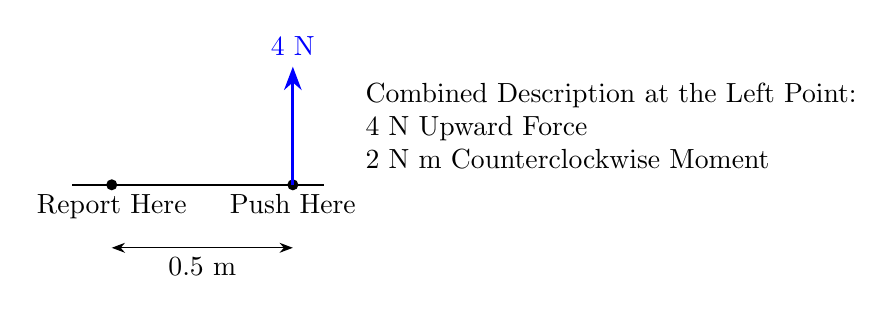
\begin{tikzpicture}[>=Stealth]
\draw[thick] (0,0)--(3.2,0);\fill(.5,0) circle(2pt);\fill(2.8,0) circle(2pt);
\node[below] at(.5,0){Report Here};\node[below] at(2.8,0){Push Here};
\draw[->,very thick,blue] (2.8,0)--(2.8,1.5) node[above]{$4$ N};
\draw[<->] (.5,-.8)--(2.8,-.8) node[midway,below]{$0.5$ m};
\node[align=left,anchor=west] at(3.6,.75){Combined Description at the Left Point:\\$4$ N Upward Force\\$2$ N m Counterclockwise Moment};
\end{tikzpicture}
\caption{An Offset Push Has Both a Resultant Force and a Moment About the Reporting Point.}
\end{figure}

The moment is mechanically real. What is unsupported is the additional claim that the player must have applied a separate twisting couple at the reporting point. A hand can apply distributed forces that form a couple, and an offset push can also create a moment. The net result alone does not distinguish those mechanisms.

This distinction is useful when discussing the grip midpoint. The midpoint is a convenient reporting location; the model does not have to claim that all finger forces physically act there. Treating an equivalent representation as a literal instruction to ``pull this much here and twist this much here'' adds an assumption that needs evidence.

\section{Why a Torque Sign Can Change Without a New Swing}
Move the reporting point to the right while leaving the actual loads unchanged. For an upward resultant, its moment about the new point decreases. In a chosen example with a $40$ N upward resultant and a $2$ N m moment at the midpoint, the reports are:
\begin{center}\begin{tabular}{lr}\toprule
Reporting Location & Moment (N m)\\\midrule
$0.10$ m Left of Midpoint & $+6$\\
Midpoint & $+2$\\
$0.10$ m Right of Midpoint & $-2$\\\bottomrule
\end{tabular}\end{center}
All three describe the same load. The sign change does not show that the lead hand twisted positively while the trail hand twisted negatively. It also does not mean the original calculation was wrong.

This is a deterministic change of reference, not an error bar. If the reporting point itself is uncertain, its uncertainty can be propagated into the moment. If the question concerns the actual contact distribution, additional assumptions or measurements are needed. Moving a reference point along the grip does not reveal where the fingers pressed.

The full three-dimensional case is richer still. A wrench can contain a residual twisting moment that cannot be eliminated by choosing a different point for a single force. A pressure center is therefore not always enough to describe the complete hand contact.

\section{Two Hands Leave Room for Hidden Load Sharing}
There is a simple example of load sharing that the rigid club motion cannot see. Add a force from one contact toward the other, and an equal force from the other contact back along the same line. The added forces cancel, and because they are collinear they add no moment. The combined club wrench is unchanged, but hand and tissue loads can change.

The words ``along the same line'' matter. Two opposite forces across a separation can create a couple. They are not automatically invisible just because they point in opposite directions. Likewise, arbitrary changes in which hand supplies an upward force usually change the moment unless another contact component compensates.

Actual contacts have limits: friction, compression, available contact area and the ability to transmit a twisting moment. A computer can select one mathematical allocation, but that selection is not a measurement of what the golfer did. An instrumented grip or independently validated contact model can add the missing information.

The mechanical loop is completed through the arms and torso as well as the club. This resembles a humanoid robot holding one object with both hands: object motion constrains the combined load but may leave internal loading undetermined. The contact model and available measurements decide how much can be recovered.

\section{Gravity Is Already in the Calculation}
It is tempting to say that inverse dynamics gives the total load and that we must subtract a second ``drift'' load to obtain the active part. Standard inverse dynamics already accounts for gravity and the inertial terms declared in its model.

Consider a simple pendulum released at an angle. It accelerates under gravity even when pivot torque is zero. A correct inverse calculation applied to that motion returns zero pivot torque. Hold the same pendulum stationary at the same angle, and the calculation instead returns the torque needed to oppose gravity. It does not confuse the first motion with active acceleration.

What it cannot automatically identify is how a person's muscles and passive tissues produced a recovered net joint torque. Opposing muscle forces can partly cancel. An omitted tissue contribution can appear in the residual load. Those are allocation and model questions, not a reason to subtract gravity twice.

A ``zero-input'' simulation also needs a definition. Setting one modeled torque to zero, keeping an identified stiffness unchanged, and asking a person to relax are different interventions. Relaxation may change posture, grip contact and feedback. A simulated zero-torque swing is a useful model comparison, not a direct demonstration of an effortless human swing.

\section{Large Force, Small Power and Real Effort Can Coexist}
Force and moment together determine how much mechanical power the hands deliver to a rigid club. When the reporting point moves, the portions assigned to force and moment can change, but their sum stays the same if the velocities are transformed consistently.

Return to the $4$ N force half a meter from the reporting point. If that point is stationary and the club rotates at $2$ rad/s, the force application point moves at $1$ m/s. The force delivers $4$ W there. At the stationary reporting point, the same power is described as $2$ N m of moment times $2$ rad/s. One description calls it force power and the other moment power; the transferred energy is identical.

Now imagine a mass moving in a circle on a rod. An inward rod force redirects its velocity. That force can be large while doing zero instantaneous work on the mass because it is perpendicular to the velocity. The force is still transmitted through the rod. An outward centrifugal term used in a rotating-frame calculation is not an extra physical load to subtract from grip tension to estimate what someone feels.

Muscle effort and perceived load need further physiological evidence. Holding a weight still can require effort despite zero external mechanical power. Co-contraction can increase tissue forces without a corresponding increase in the net torque. For a real golf club, moving hands and shaft deformation further complicate the power balance.

\section{Air Resistance Is a Model Question, Not a Universal Correction}
An aerodynamic force acts with a direction and a moment arm. Omitting it biases the inferred hand force and moment. Its effect on a signed torque component can go either way, and its percentage effect can be large when that component is close to zero.

The long technical companion reconstructs the original handwritten example with explicit axes. For one assumed air-force direction, the transverse hand-force magnitude falls from $7.5$ to $5.5$ pounds-force and the negative moment magnitude falls by about $39.9\%$. Reversing that air-force direction increases both magnitudes. The original reduction is mechanically possible; its value depends on the assumed load, geometry and reporting point. The saved video stills establish some displayed numbers but do not establish the assumed seven-iron drag.

A study of driver-head aerodynamic features provides evidence for that equipment and test configuration. It does not establish the drag of a seven-iron or a universal correction to every torque curve. Drag opposes relative airflow; lift and aerodynamic couples also matter. The relevant question is whether plausible aerodynamic uncertainty changes the particular conclusion being drawn.

\section{How to Use the Evidence in Coaching}
Start with the outcome you want to understand: club delivery, ball flight, joint load, transferred work or felt effort. Then identify what the available measurement actually constrains. A launch-monitor result describes the end of a chain involving body motion, ground contact, the grip, shaft deformation and collision; it does not uniquely reconstruct the chain.

For a named quantity such as ``alpha torque,'' ask for the reporting point, axes, positive direction and action convention before comparing signs. Compare swings under consistent definitions, equipment and processing. Examine whether the claimed difference survives plausible measurement, filtering and model changes.

A proposed mechanism should make a testable prediction. For example, a hand-path change might alter speed through additional work, through changed energy distribution, or both. Computing complete work and stored energy helps distinguish those possibilities. A large force normal to the hand path or a sequence of velocity peaks cannot settle the question alone.

Use independent measurements to test the interpretation. A force estimate outside calibrated grip-sensor uncertainty, an impossible contact allocation or a work balance that does not close is useful evidence against the current explanation. Treat the result as a reason to improve the model or the measurement, rather than as a cue about how the golfer ought to feel.

\section*{Further Reading}
The companion \emph{Interpretation of Inverse Dynamics: Understanding the Fundamental Limitations} gives the full balances, worked numbers and research-source limits. Standard wrench mechanics is developed in K. M. Lynch and F. C. Park, \emph{Modern Robotics} (2017), Chapter 3; its accessible supplement is \url{https://modernrobotics.northwestern.edu/nu-gm-book-resource/3-4-wrenches/}. The practical distinction throughout this guide is between a net mechanical estimate and the additional evidence needed to explain contact strategy, muscle activity or sensation.
\end{document}
